% UFFS presentation theme
% 2016-06-21 - Rafael Hengen Ribeiro - rafaelhr.ribeiro@gmail.com
%   Baseado no tema do IFSC: 2015-05-21 - Emerson Ribeiro de Mello - mello@ifsc.edu.br

\documentclass[t,aspectratio=169]{beamer} % Aspecto 16:9 (WIDESCREEN)
%\documentclass[t]{beamer} % Aspecto 4:3

\usepackage[utf8]{inputenc}
\usepackage[T1]{fontenc}
\usepackage[english,brazil]{babel}
\usepackage{hyperref}
\usepackage[alf]{abntex2cite}	% Citações padrão ABNT

\usepackage{tikz}

% usando tema personalizado. 
% arquivo beamerthemeUFFS.sty deve estar no mesmo diretório do .tex
\usepackage{beamerthemeUFFS}
\usepackage{ragged2e}

% Metadados do PDF
\hypersetup{pdfstartview={Fit},
    pdftitle={Modelo de apresentação do curso de Ciência da Computação da UFFS},
 	pdfsubject={assunto},
 	pdfauthor={Rafael Hengen Ribeiro}
}

%%%%%%%%%%%%%%%%%%%%%%%%%%%%%%%%%%%%%%%%%%%%


\title{Modelo de apresentação}
\author{Rafael Hengen Ribeiro}

%\date{28 de junho de 2016} % Se não especificar, fica a data da compilação
\institute{Curso de Ciência da Computação\\
Universidade Federal da Fronteira Sul\\
Campus Chapecó}



%%%%%%%%%%%%%%%%%%%%%%%%%%%%%%%%%%%%%%%%%%%%

\begin{document}

\addtobeamertemplate{frametitle}{}{%
\begin{tikzpicture}[remember picture,overlay]
\node[anchor=north east,yshift=2pt] at (current page.north east) {
\includegraphics[height=1cm]{logo_curso}};
\end{tikzpicture}}

\setbeamertemplate{footline}{ 
	\color{white}
     \\
    }

\begin{frame}
	\maketitle
\end{frame}

\addtocounter{framenumber}{-1}
% Descomente as linhas abaixo se desejar colocar um sumário de todas as seções
%\begin{frame}[t]{Sumário}
%\tableofcontents
%\end{frame}
\setbeamertemplate{footline}{
    \color{black}
    \hfill \insertframenumber\,/\,\inserttotalframenumber~
}

\def\sectionname{}
\def\insertsectionnumber{}
\def\subsectionname{}
\def\insertsubsectionnumber{}

\AtBeginSection{\frame{\sectionpage}\addtocounter{framenumber}{-1}}


\AtBeginSubsection{\frame{\subsectionpage}\addtocounter{framenumber}{-1} }
\AtBeginSubsubsection{\frame{\subsubsectionpage}\addtocounter{framenumber}{-1} }


%%%%%%%%%%%%%%%%%%%%%%%%%%%%%%%%%%%%%%%%%%%%
% Inicio do documento
%%%%%%%%%%%%%%%%%%%%%%%%%%%%%%%%%%%%%%%%%%%%

% SLIDES
\begin{frame}{Introdução - Listas}
    Listas
    \begin{itemize}
        \item Item 1
        \begin{itemize}
            \item Subitem 1
        \end{itemize}
        \item Citação - \cite{vasisht2016}
    \end{itemize}
    

    Lista enumerada
    \begin{enumerate}
        \item Item enumerado 1
        \begin{enumerate}
            \item Subitem enumerado 1
        \end{enumerate}
    \end{enumerate}
\end{frame}
\begin{frame}[fragile]{Código em C e Python}
    \ansic
	\begin{lstlisting}
	 int main(void){
	    printf("Ola mundo\n");
	    return 0;
	 }
	\end{lstlisting}

    \python
	\begin{lstlisting}
	def funcao():
	   print("Teste")
	\end{lstlisting}	
	
\end{frame}


\begin{frame}{Imagens}
    \begin{figure}
        \centering
        % height=0.65\textheight -> 65% da altura do texto/slide
        % width=0.4\textwidth -> 40% da largura do texto/slide
        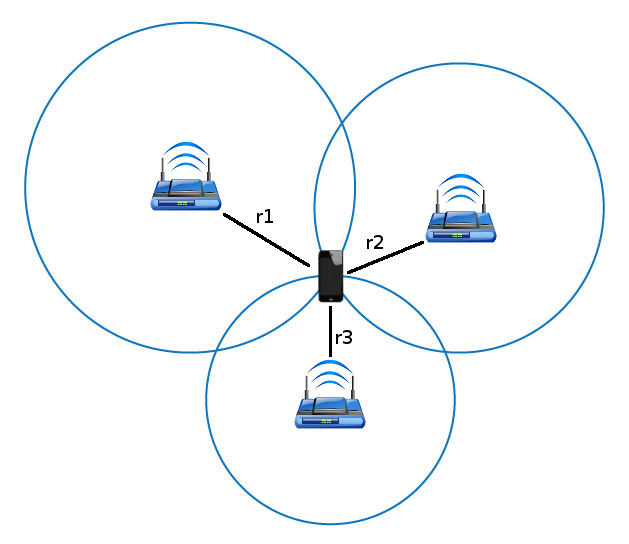
\includegraphics[height=0.65\textheight]{img/trilateration}
        \caption{Texto abaixo da imagem}
        \label{fig:trilateration}
    \end{figure}
\end{frame}


%%%%%%%%%%%%%%%%%%%%%%%%%%%%%%%%%%%%%%%%

\setbeamertemplate{footline}{ \color{white}\\}
\addtocounter{framenumber}{-1}

% Para Referências grandes descomente a linha abaixo
%\begin{frame}[allowframebreaks]{Referências} 
\begin{frame}{Referências}
    \bibliography{referencias}
\end{frame}

%%%%%%%%%%%%%%%%%%%%%%%%%%%%%%%%%%%%%%%%%%
% Para REPETIR CAPA NO FINAL 
%   descomente as linhas abaixo
%%%%%%%%%%%%%%%%%%%%%%%%%%%%%%%%%%%%%%%%%
%\addtocounter{framenumber}{-1}
%\begin{frame}
%	\maketitle
%\end{frame}

\end{document}